\documentclass[answers,12pt,addpoints]{exam}
\usepackage{graphicx,multicol}
\usepackage{charter,amsmath,amssymb}
\usepackage{eulervm}
\usepackage[letterpaper,margin=1in]{geometry}
\pagestyle{headandfoot}
\runningheadrule
\runningheader{\bf Math 265}
{\bf Exam Two, Page \thepage\ of \numpages}
{\bf 4 March 2015}
\firstpagefooter{}{}{}
\runningfooter{}{}{}
\let\cos\relax\DeclareMathOperator{\cos}{\mathsf{cos}}
\let\sin\relax\DeclareMathOperator{\sin}{\mathsf{sin}}
\let\ln\relax\DeclareMathOperator{\ln}{\mathsf{ln}}
\let\lim\relax\DeclareMathOperator*{\lim}{\mathsf{lim}}
\everymath{\displaystyle}
\begin{document}
\begin{center}
\huge Math 265 Exam Two\\
\LARGE Spring 2015
\end{center}

\ifprintanswers\else
\begin{center}
\fbox{\fbox{\parbox{5.5in}{
This exam has \numquestions~questions.
It has been printed on \numpages~pages and is worth \numpoints~points.
Answer all the questions in the spaces provided.
%The last page has been left blank for your calculations.
Although you may use any calculator on this exam,
you must clearly indicate how you arrived at your answers
in order to receive maximum credit.
By signing below, you pledge that you
\begin{enumerate}
\item will not communicate to any person in any conceivable way anything
about the contents of this exam
until all students have taken it, and
\item have not been the recipient of such communication from anyone else.
\end{enumerate}}}}
\end{center}
\vspace{.2in}
\makebox[\textwidth]{Your signature:\enspace\hrulefill}\\
\vspace{.2in}\\
\makebox[\textwidth]{Your name:\enspace\hrulefill}\\
\begin{center}\gradetable[h][questions]\end{center}
\fi

\begin{questions}

\begin{multicols}{2}
\question[25] Find and classify all
the critical points of \[f\left(x,y\right)
=x^3+y^3-3x-3y\] as local maxima, local minima,
saddle points, or none of these.
The contour plot of $f$ is shown at the right.
\begin{center}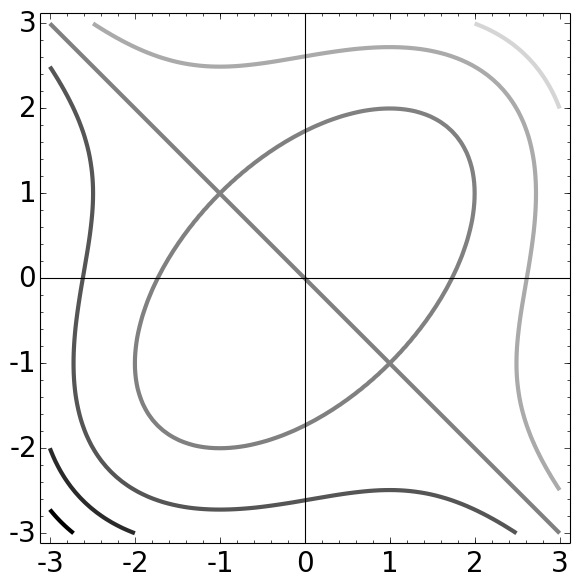
\includegraphics[scale=.4]{Saddles}\end{center}
\end{multicols}

\begin{multicols}{2}
\question[25] Calculate the curvature
$\kappa\left(t\right)$ of the curve
\[\mathbold{r}\left(t\right)
=\left\langle\cos^3\left(t\right),\sin^3\left(t\right)
\right\rangle\]
shown at the right.
\begin{center}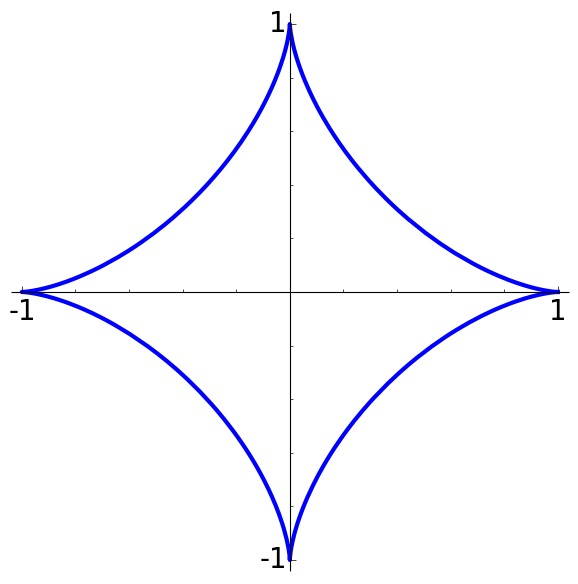
\includegraphics[scale=.4]{Astroid}\end{center}
\end{multicols}

\question[25] Imagine that you are walking on the surface
$z=x^2+4y^2+1$ directly above the curve in the
$xy$-plane given by $\mathbold{r}\left(t\right)
=\left\langle\cos{t},\sin{t}\right\rangle$
for $0\le t\le 2\pi$
in the direction of increasing~$t$.
\begin{parts}
\part Calculate $z'\left(t\right)$.
\part Find the values
of $t$ for which you are walking uphill. That is,
find the values of $t$ where $z$ is increasing.
\end{parts}

\question[25] The temperature of a gas at the point
$\left(x,y,z\right)$ is given by $G\left(x,y,z\right)
=x^2-5xy+y^2z$.
\begin{parts}
\part What is the rate of change in the temperature
at the point $\left(1,2,3\right)$ in the direction
$v=2\mathbold{i}+\mathbold{j}-4\mathbold{k}$?
\part In which direction is temperature increasing
fastest at the point $\left(1,2,3\right)$?
\part What is the maximum rate of change of temerature
at the point $\left(1,2,3\right)$?
\end{parts}

\end{questions}
\end{document}
